\chapter{Część aplikacyjna - program umożliwiający sprawdzanie obecności przy pomocy biometrycznego systemu kontroli dostępu}
\label{cha:systemKontroli}

W rozdziale dotyczącym części aplikacyjnej opisany zostanie interfejs użytkownika systemu sprawdzania obecności na zajęciach, wraz z bazą danych przechowującą informacje niezbędne do identyfikacji lub weryfikacji tożsamości osób. Program ten stanowi rozwiniętą formę aplikacji opisanej w pracy \cite{Gl11}, oferującą zaawansowane funkcje operowania na bazie danych, zaproponowane w \cite{Gl11} jako kierunek dalszego rozwoju systemu.

\section{Interfejs aplikacji}
\label{sec:aplikacja}

Podstawowa wersja opisywanego systemu sprawdzania obecności na zajęciach zapewniała minimum funkcji koniecznych do korzystania z programu. Wśród możliwości tych znajdowały się takie opcje, jak:
\begin{itemize}
\item pobranie dynamicznego lub statycznego obrazu przy pomocy kamery
\item zapis pobranego obrazu w wybranej lokalizacji
\item wczytanie zdjęcia oka ludzkiego, zapisanego uprzednio na dysku twardym
\item zaprezentowanie działania poszczególnych etapów algorytmów, wykrywających tęczówkę oraz tworzących kod na podstawie przetwarzanych danych
\item wprowadzenie do bazy nowego użytkownika poprzez uzupełnienie danych osobowych (imię, nazwisko, kierunek studiów, grupa)
\item identyfikację istniejącego już użytkownika w oparciu o analizowane dane
\end{itemize}

Aplikacja rozwinięta na potrzeby niniejszej pracy została wzbogacona o funkcje umożliwiające zaawansowane wykorzystanie zalet oferowanych przez biometryczny system kontroli dostępu i sprawdzania obecności. Proponowany schemat działania programu w przypadku uzupełnienia o tego rodzaju możliwości został przedstawiony w \cite{Gl11}. Na diagramie \ref{fig:program} zaprezentowano zaktualizowaną wersję schematu, uwzględniającą funkcje dodane w zaawansowanej wersji programu.

\begin{figure}
\begin{center}
\label{fig:program}
\end{center}
\end{figure}

Opis dodanych możliwości korzystania z aplikacji przedstawiono w dalszej części pracy.

Interfejs użytkownika systemu został rozwinięty o zbiór specjalnych zakładek, pozwalających na wprowadzanie danych do bazy zgodnie ze schematem na rysunku \ref{fig:program}. Dostępne są one po naciśnięciu przycisku Zaawansowane opcje dodawania, widocznym na rysunku \ref{fig:oknoGlowne}. 

Pierwszą zakładką, umożliwiającą uzupełnienie bazy o nowe informacje, jest Dodaj kierunek, pokazana na rysunku \ref{fig:dodajSpecjalizacje}. Składa się ona z pól Nazwa kierunku i Nazwa wydziału. W celu dodania nowego kierunku do bazy, należy uprzednio wprowadzić nazwę wydziału, z którym kierunek będzie powiązany, a następnie zatwierdzić zmiany. Po wybraniu wydziału z listy, można wpisać nazwę kierunku. Aby zmodyfikować istniejący kierunek, należy wybrać z listy rozwijalnej nazwę wydziału, a następnie nazwę zmienianego kierunku. Pola zakładki zostały wyposażone w podpowiedzi, pełniące funkcje pomocy w przypadku, gdy użytkownik nie jest pewny, jakiej postaci powinny być wpisywane dane. 
\begin{figure}
\begin{center}
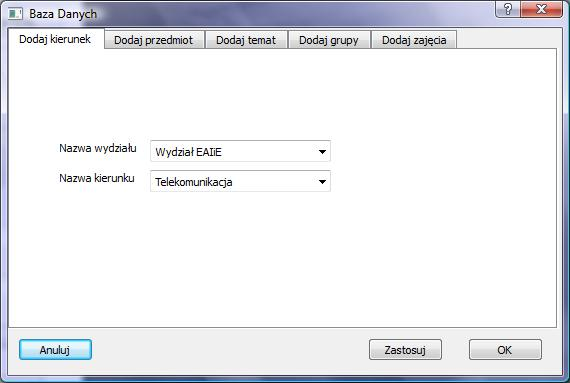
\includegraphics[scale=0.7]{dodaj_kierunek.jpg}
\caption{Zakładka do dodawania wydziałów i kierunków}
\label{fig:dodajSpecjalizacje}
\end{center}
\end{figure}

Następną zakładką dającą możliwość wprowadzania danych jest Dodaj przedmiot. Posiada ona pola Wydziału, Kierunku, Nazwy przedmiotu oraz Roku studiów, w trakcie którego przedmiot jest prowadzony. Nazwy wydziału i kierunku można wybrać z list rozwijalnych. Po wybraniu wydziału, istnieje możliwość wyboru wyłącznie kierunków związanych z danym wydziałem. W celu zmiany danych istniejącego w bazie przedmiotu, można wybrać go z listy w polu Nazwy przedmiotu, wówczas pole Rok studiów ulegnie uzupełnieniu informacjami. Podobnie jak w przypadku dodawania kierunku, również w tej zakładce dostępna jest pomoc dla użytkownika w postaci pojawiających się podpowiedzi. 
\begin{figure}
\begin{center}
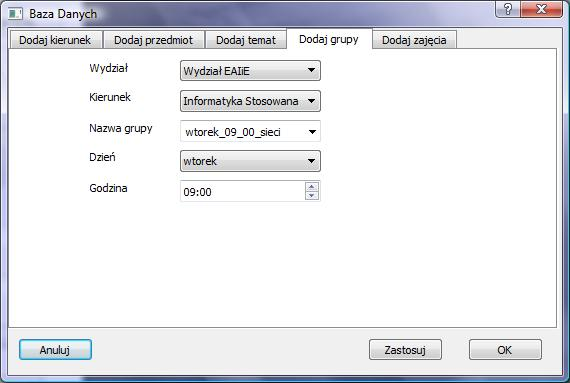
\includegraphics[scale=0.7]{dodaj_grupe.jpg}
\caption{Zakładka do dodawania grup}
\label{fig:dodajGrupe}
\end{center}
\end{figure}

\begin{figure}
\begin{center}
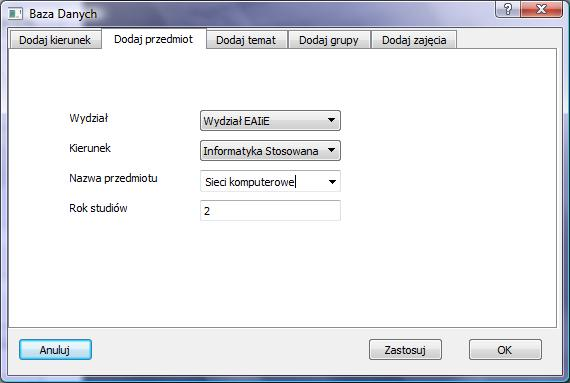
\includegraphics[scale=0.7]{dodaj_przedmiot.jpg}
\caption{Zakładka do dodawania przedmiotów}
\label{fig:dodajPrzedmiot}
\end{center}
\end{figure}

W zakładce Dodaj temat, obecnej na rysunku \ref{fig:dodajTemat}, możliwe jest dodawanie tematów realizowanych w obszarze danego przedmiotu. Dostępne pola na tej zakładce to Wydział, Kierunek, Przedmiot oraz Nazwa tematu. Pole nazwy tematu należy uzupełnić wybranymi danymi. W przypadku edycji istniejącego tematu, można wybrać go z listy takiej, jak w polach nazw wydziału, kierunku i przedmiotu.

\begin{figure}
\begin{center}
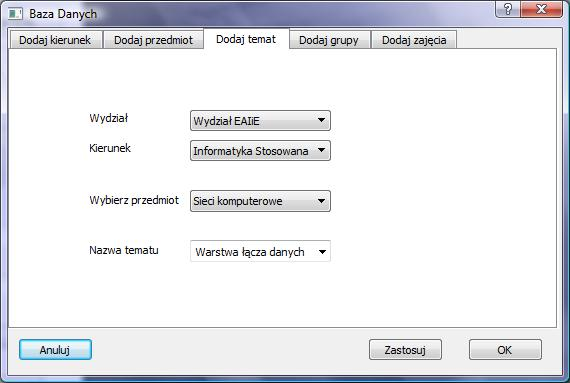
\includegraphics[scale=0.7]{dodaj_temat.jpg}
\caption{Zakładka do dodawania tematów}
\label{fig:dodajTemat}
\end{center}
\end{figure}

\begin{figure}
\begin{center}
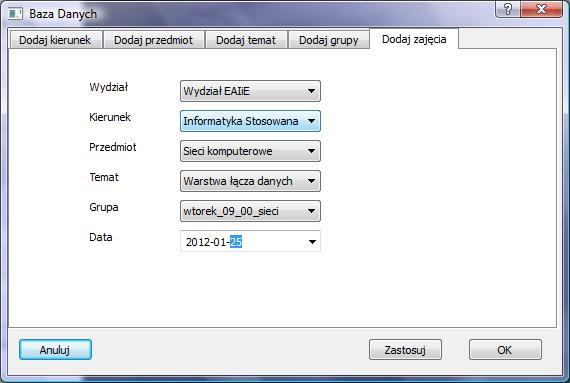
\includegraphics[scale=0.7]{dodaj_zajecia.jpg}
\caption{Zakładka do dodawania zajęć}
\label{fig:dodajZajecia}
\end{center}
\end{figure}
Kolejna zakładka o nazwie Dodaj grupę, umożliwia tworzenie grup studentów uczęszczających na zajęcia z przedmiotów. Pola niezbędne do wypełnienia na niej to Wydział, Kierunek, Przedmiot, Dzień odbywania się zajęć (do wybrania z listy dni tygodnia), Godzina odbywania się zajęć (w formie GG:MM, gdzie GG odpowiada godzinie, a MM minutom), oraz Nazwa grupy. W przypadku nazwy tej wymagane jest, aby była ona różna od wszystkich innych nazw grup obecnych w bazie.

Następna zakładka pozwalająca na uzupełnienie bazy danych to Dodaj zajęcia. Obecne na niej pola Wydziału, Kierunku, Przedmiotu oraz Grupy umożliwiają wprowadzenie do bazy zajęć odbywających się w terminie wybranym w polu Data zajęć, podczas których realizowany będzie określony temat. W zakładce tej również pojawiają się podpowiedzi informujące o formie wprowadzanych nazw i daty.

\begin{figure}
\begin{center}
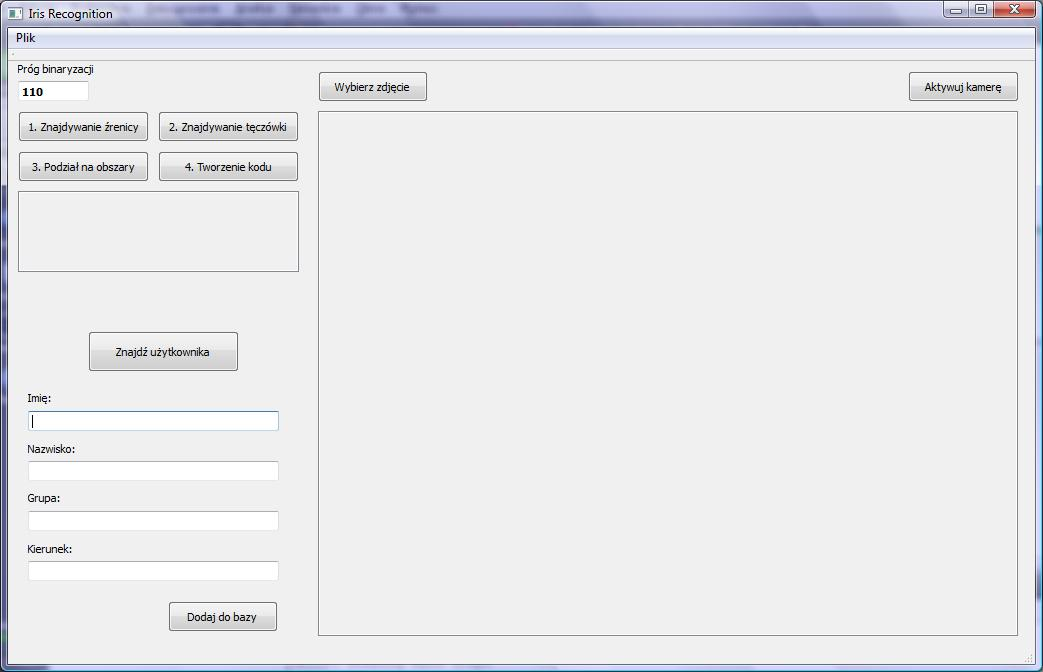
\includegraphics[scale=0.5]{okno_glowne.jpg}
\caption{Główne okno programu}
\label{fig:oknoGlowne}
\end{center}
\end{figure}

\begin{figure}
\begin{center}
\label{fig:wybraneTabele}
\end{center}
\end{figure}

Po uzupełnieniu bazy kierunkami, przedmiotami, grupami, tematami i zajęciami można przystąpić do dodawania użytkowników. W tym celu potrzeba wypełnić w oknie głównym programu pola Imię, Nazwisko, Kierunek i Grupa, w formie ręcznego wprowadzania danych bądź wyboru informacji z listy.

Możliwe jest również wprowadzenie użytkowników bez wcześniejszego uzupełnienia kierunków, przedmiotów i grup, ale wymaga to późniejszej modifikacji informacji w zakładkach w celu zachowania spójności danych w bazie.

Aby przypisać użytkownikowi biometrykę, należy postępować zgodnie ze schematem przedstawionym w dalszych częściach pracy.

Pierwszym wymaganym krokiem jest opisane uzupełnienie danych użytkownika. Niezbędne jest również pobranie zdjęcia dodawanego użytkownika lub wczytanie  go z nośnika danych. Następnie należy wcisnąć przycisk Dodaj do bazy. Spowoduje to otwarcie okienka z wynikiem segmentacji obszaru tęczówki, który powinien być zweryfikowany przez użytkownika. Po pozytywnej weryfikacji utworzony zostaje kod tęczówki danej osoby.

W celu sprawdzenia obecności użytkowników, wymagane jest pobranie zdjęć poszczególnych osób i wyznaczenie kodów potrzebnych do ich identyfikacji. W przypadku pozytywnej identyfikacji danej osoby pola danych osobowych ulegają uzupełnieniu. Można wówczas wybrać zajęcia, na których obecna jest osoba, oraz ewentualnie temat odrabianych zajęć, jeśli jest to student odrabiający. W przypadku nierozpoznania osoby, informacje nie są uzupełniane i nie można przypisać użytkownika do zajęć w bazie.
Program umożliwia również generację list obecności na danych zajęciach. Funkcja ta jest dostępna przy użyciu przycisku Generuj listę obecności.
\section{Baza danych}
\label{sec:bazadanych}

Program opisany w pracy \cite{Gl11} działał w oparciu o nieskomplikowaną bazę danych, składającą się z pojedynczej tabeli o polach id, name, surname, group, faculty, iris\_code. Taki układ bazy sprzyjał niskiej złożoności wykonywanych operacji, prostocie zapytań wysyłanych do bazy oraz dużej szybkości działania programu. Było to związane z brakiem konieczności łączenia tabel dla uzyskania informacji dotyczących użytkownika. Jednocześnie jednak taka budowa ograniczała rozszerzenie opcji aplikacji, które umożliwiałyby wiązanie kierunków z przedmiotami, a przedmiotów z grupami studentów oraz konkretnymi zajęciami. W związku z zaistniałą niedogodnością, w aplikacji rozwiniętej na potrzeby niniejszej wersji systemu podjęto próbę utworzenia rozbudowanej bazy danych.

Schemat przebudowanej bazy przedstawiony jest na diagramie \ref{fig:bazaDanych}.

 
\begin{figure}
\begin{center}
\label{fig:bazaDanych}
\end{center}
\end{figure}

Baza ta składa się z tabel, których funkcją jest logiczne usegregowanie informacji wprowadzanych do systemu podczas procesu przyporządkowywania studentów poszczególnym kierunkom, przedmiotom i grupom, biorącym udział w zajęciach obejmujących wybraną tematykę. Uzupełnianie danych w bazie dzieli się na etapy wyszczególnione na diagramie \ref{fig:etapyDzialania}, który został oparty na schemacie zaprezentowanym w pracy \cite{Gl11}.

\begin{figure}
\begin{center}
\label{fig:etapyDzialania}
\end{center}
\end{figure}

W przypadku uruchamiania systemu biometrycznej kontroli dostępu po raz pierwszy, możliwe jest jedynie dodawanie użytkowników do bazy w sposób podstawowy, niezapewniający funkcji przyporządkowywania osób istniejącym kierunkom, przedmiotom i grupom. Jest to spowodowane początkowym brakiem danych w tabelach odpowiedzialnych za przechowywanie niesionych z tym informacji. Wypełnienie pól znajdujących się w głównym oknie aplikacji, przedstawionym na obrazku \ref{fig:oknoGlowne}, powoduje uzupełnienie wyłącznie wybranych atrybutów w tabelach Students, Biometrics, Groups i Faculties (rysunek \ref{fig:wybraneTabele}). 

Aby w pełni wykorzystać możliwości systemu, należy wprowadzać informacje przy pomocy specjalnych zakładek opisanych szczegółowo w części \ref{sec:aplikacja}. Uzupełnianie danych w ten sposób pozwala na postępowanie zgodnie ze schematem \ref{fig:etapyDzialania}, co umożliwia późniejszy szybki wybór oraz modyfikację informacji umieszczonych w bazie i generowanie gotowych list obecności na zajęciach.

Opis danych wprowadzanych do bazy podczas wypełniania pól na kolejnych zakładkach został przedstawiony poniżej.

Pierwszą zakładką, w której możliwe jest wprowadzenie danych do bazy, jest Dodaj kierunek, ukazana na rysunku \ref{fig:dodajSpecjalizacje}. W trakcie dodawania kierunku bądź edycji już istniejącego, wraz z wypełnieniem pól i potwierdzeniem wpisywanych informacji, uzupełniane lub modyfikowane są następujące atrybuty:

W tabeli Wydziały (Faculties):

\begin{itemize}
\item Nazwa wydziału (faculty) - pole z nazwą wydziału
\item Identyfikator wydziału (faculty\_id) - pole z unikatowym identyfikatorem wydziału
\end{itemize}

W tabeli Kierunki:

\begin{itemize}

\item Kierunek (specialisation) - jest to pełna nazwa kierunku; pole to jest jednym z wymaganych przy wprowadzaniu informacji 
\item Wydział (faculty\_id) - identyfikator wydziału; pole jest wymagane
\item Identyfikator kierunku (specialisation\_id) - jest to unikalne pole, identyfikujące kierunek wśród innych w sposób jednoznaczny; nie wymaga ono bezpośredniego wprowadzania wartości przez użytkownika, gdyż jest automatycznie uzupełniane przy tworzeniu nowego rekordu, dlatego też w interfejsie aplikacji nie ma specjalnego miejsca dla wprowadzenia danych odnoszących się do niego
\end{itemize}
Kolejną zakładką umożliwiającą uzupełnienie bazy danych jest Dodaj przedmiot, przedstawioną na rysunku \ref{fig:dodajPrzedmiot}. Podczas wprowadzania przedmiotu lub edycji informacji dotyczących istniejącego, w efekcie potwierdzenia danych wpisanych w odpowiednich polach, uzupełnieniu ulegają następujące atrybuty tabeli Przedmioty (Subjects):
\begin{itemize}
\item Przedmiot (subject) - pełna nazwa przedmiotu; jest to pole wymagane
\item Kierunek (specialisation\_id) - pole zawierające identyfikator kierunku, na którym prowadzony jest przedmiot; jest ono uzupełniane poprzez wybranie nazwy kierunku i wydziału z listy, które są przekształcane na odpowiedni identyfikator charakteryzujący kierunek w tabeli Kierunki
\item Rok studiów (year\_of\_studies) - rok studiów kierunku, podczas którego prowadzony jest dany przedmiot
Identyfikator przedmiotu (subject\_id) - jest to unikalny identyfikator dla przedmiotu w obrębie tabeli
\end{itemize}

Używając zakładki Dodaj temat, przedstawionej na rysunku \ref{fig:dodajTemat}, można wprowadzić do bazy dane dotyczące tematów realizowanych w obrębie istniejących w bazie przedmiotów. Po uprzednim wypełnieniu pól i zatwierdzeniu wpisywanych informacji, uzupełniane są następujące atrybuty tabeli Tematy (Topics):
\begin{itemize}
\item Temat (topic) - pełna nazwa wprowadzanego tematu
\item Przedmiot (subject\_id) - pole identyfikatora przedmiotu, w obrębie którego dodawany jest temat; po wybraniu przez użytkownika nazwy przedmiotu, kierunku, wydziału i roku, na których jest prowadzony, następuje wyszukanie odpowiadającego im identyfikatora w tabeli Przedmioty
\item Identyfikator tematu (topic\_id) - unikalny identyfikator tematu, automatycznie tworzony podczas wprowadzania danego tematu; nie wymaga on bezpośredniego wpisywania danych przez użytkownika, dlatego nie posiada odpowiadającego mu pola w aplikacji
\end{itemize}

Uzupełniając zakładkę Dodaj grupę, możliwe jest wprowadzenie grup studentów, na które zostaną podzieleni w obrębie danego przedmiotu. Zakładka przedstawiona została na rysunku \ref{fig:dodajGrupe}. Wraz z potwierdzeniem wpisywanych informacji, do bazy wprowadzeniu ulegają wartości następujących atrybutów tabeli Grupy (Groups):
\begin{itemize}
\item Identyfikator przedmiotu (subject\_id) - pole zawierające informacje na temat przedmiotu, w obrębie którego tworzona jest dana grupa; na podstawie wybranych informacji wyszukiwany jest identyfikator przypisany do przedmiotu w tabeli Przedmioty
\item Dzień odbywania się zajęć (day\_of\_week) - dzień tygodnia, w którym odbywać się będą zajęcia grupy
\item Godzina odbywania się zajęć (time\_of\_classes) - godzina odbywania się zajęć danej grupy
\item Nazwa grupy (group\_name) - nazwa grupy; musi ona być unikalna w całej tabeli Grupy
\item Identyfikator grupy (group\_id) - identyfikator jednoznacznie określający grupę w tabeli; jest to wartość tworzona automatycznie, nie wymaga wprowadzania informacji od użytkownika.
\end{itemize}

Aby przypisać użytkowników do grup, należy powrócić do okna głównego aplikacji, w którym znajdują się pola służące do wprowadzania danych osobowych. Po uzupełnieniu pól, odpowiednim atrybutom tabel Studenci (Students) oraz Grupy studentów (Students\_Groups) nadawane są wartości:

W tabeli Studenci:
\begin{itemize}
\item Imię (name) - pełne imię użytkownika
\item Nazwisko (Surname) - pełne nazwisko studenta
\item Kierunek (specialisation\_id) - informacje dotyczące kierunku studiów; po wybraniu opcji z listy kierunków umieszczonych w bazie Kierunki, przyporządkowany zostaje identyfikator kierunku, opisujący go w sposób unikalny
\item Przedmiot (subject\_id) - dane przedmiotu, do którego zostanie przypisany student; wybrane informacje ulegają przekształceniu na identyfikator przedmiotu w tabeli Przedmioty
\item Grupa (group\_id) - nazwa grupy z przedmiotu, do której będzie przypisany student; na podstawie nazwy tej uzupełniany jest identyfikator danej grupy
\item Identyfikator studenta (student\_id) - unikalny identyfikator dla osoby w obrębie całej tabeli
\item Identyfikator biometryki (biometrics\_id) - identyfikator biometryki, tworzonej dla każdego studenta
\end{itemize}

W tabeli Grupy studentów:
\begin{itemize}
\item Identyfikator grupy (group\_id) - identyfikator grupy przedmiotu
\item Identyfikator studenta (student\_id) - identyfikator studenta, który jest tworzony i automatycznie przypisywany do grupy o wymienionym identyfikatorze group\_id
\end{itemize}

Podstawową funkcją tabeli Grupy studentów jest połączenie informacji przechowywanych w tabelach Studenci oraz Grupy. Podczas dodawania kolejnych osób do grupy o danej nazwie, następuje uzupełnianie tabeli Grupy studentów rekordami o tym samym identyfikatorze grupy, ale różnych identyfikatorach studentów, co powoduje przypisanie wielu osób do tej samej grupy. 

Wśród najważniejszych funkcji stworzonego systemu można wyróżnić tworzenie kodu tęczówki oka dla każdego użytkownika oraz przechowywanie go w specjalnie do tego przygotowanych strukturach danych. Tabelą gromadzącą kody tęczówek jest tabela Biometryki (Biometrics). Składa się ona z następujących atrybutów:
\begin{itemize}
\item Kod tęczówki (iris\_pattern) - pole przechowujące informacje o utworzonym kodzie tęczówki 
\item Odcisk palca (fingerprint\_pattern) - dodatkowe pole przechowujące kod odcisku palca, które mogłoby być wykorzystane w przypadku rozbudowy systemu o funkcjonalność rozpoznawania na tej podstawie
\item Kod twarzy (face\_pattern) - pole przechowujące informacje dotyczące kształtu twarzy, używane w przypadku poszerzenia systemu o identyfikację w oparciu o kształt twarzy
\item Identyfikator biometryki (biometrics\_id) - identyfikator charakteryzujący biometrykę
\end{itemize}

Tabelą pomocniczą dla tabeli Biometryki jest Zdjęcia (Photos). Posiada ona atrybuty:
\begin{itemize}
\item iris\_1 .. iris\_5 - pole przechowujące pobrane zdjęcia tęczówki oka, służące do tworzenia kodu tęczówki
\item finger\_1 .. finger\_5 - pola służące do przechowywania zdjęć odcisków palca, w przypadku, gdy system zostanie poszerzony o funkcjonalność identyfikacji na podstawie odcisków palców
\item face\_1 .. face\_5 - pola przechowujące fotografie twarzy, w przypadku, gdy system posiada funkcjonalność rozpoznawania na podstawie kształtu twarzy
\end{itemize}

W celu utworzenia zajęć z przedmiotu, łączących tematy z konkretnymi terminami w postaci daty, należy wypełnić pola w zakładce Dodaj zajęcia, przedstawionej na rysunku \ref{fig:dodajZajecia}. Powoduje to uzupełnienie tabeli Zajęcia (Classes), która posiada atrybuty:
\begin{itemize}
\item Przedmiot (subject\_id) - identyfikator przedmiotu, z którego odbywać się będą zajęcia; jest on pobierany z tabeli Przedmioty na podstawie wybranego pola
\item Temat (topic\_id) - identyfikator tematu, który będzie realizowany na danych zajęciach
\item Grupa (group\_id) - identyfikator grupy, do której przypisane będą zajęcia
\item Data (class\_date) - termin zajęć
\item Kierunek (specialisation\_id) - identyfikator kierunku, w skład którego wchodzą użytkownicy z danej grupy
\item Identyfikator zajęć (class\_id) - unikalny identyfikator zajęć
\end{itemize}
Tabelami umożliwiającymi uzupełnienie list obecności oraz osób odrabiających zaległe tematy są Obecność (Attendance) i Odrabiający (Complements). Posiadają one pola:
\begin{itemize}
\item Tabela Obecność:
\begin{itemize}
\item Identyfikator zajęć (class\_id) - identyfikator zajęć, na których obecny lub nieobecny jest użytkownik
\item Identyfikator studenta (student\_id) - identyfikator użytkownika
\item Obecny (present) - logiczna wartość, wskazująca na obecność studenta
\end{itemize}
\item Tabela Odrabiający:
\begin{itemize}
\item Identyfikator zajęć (class\_id) - identyfikator zajęć, które osoba odrabia
\item Identyfikator studenta (student\_id) - identyfikator użytkownika
\item Data uzupełniania zajęć (complement\_date) - data odrabiania danych zajęć
\end{itemize}
\end{itemize}

Dodawanie informacji do tych tabel możliwe jest w przypadku, gdy osoba identyfikowana istnieje w systemie. Wówczas aktywowany zostaje przycisk Dodaj obecność, który otwiera specjalnie stworzone menu, pozwalające na wprowadzenie danych do powyższych tabel.

\section{Zastosowane technologie}
\label{sec:implementacja}

Podczas rozbudowy podstawowej wersji aplikacji użyto technologii zaproponowanych w pracy \cite{Gl11}, ze względu na oferowane przez nie zalety. Jedynie w procesie projektowania bazy danych zdecydowano się na wdrożenie odmiennej technologii. Spowodowane to było niedostępnością dodatku obsługującego MySQL w używanym środowisku programistycznym, stosowanym do zaprojektowania systemu.

Językiem programowania, użytym podczas implementacji obsługi bazy danych, był C++. Jest to rozbudowany, obiektowy język oferujący wiele różnych bibliotek, w tym pomocnej w przesyłaniu zapytań. C++ posiada bogate API, co ułatwia korzystanie z gotowych funkcji interfejsu.

Środowiskiem programistycznym służącym do tworzenia aplikacji był QtCreator, z wbudowaną biblioteką Qt w wersji. Biblioteka ta umożliwia tworzenie zaawansowanych interfejsów użytkownika przy użyciu gotowych widgetów i form, bez konieczności budowania GUI od podstaw.

Wśród wielu technologii bazodanowych, najlepszą okazała się być SQLite w wersji. Nie wymaga ona uruchamiania serwera dlatego też umożliwia przenośność aplikacji. Zdefiniowane w niej rodzaje struktur przechowywanych danych wymagają niewiele przestrzeni dyskowej oraz są intuicyjne, co ułatwia pracę z SQLite.  
